\subsection{Выбор протокола передачи данных}

Для обеспечения взаимодействия типа ``клиент-сервер'' необходимо использовать один из протоколов передачи данных.

HTTP является основным протоколом передачи данных во Всемирной паутине. Он действует как протокол типа ``запрос-ответ'' в модели клиент-серверной модели~\cite{http_websockets}.

При использовании протокола HTTP, клиент отправляет на сервер запрос и ожидает ответа. Сервер оставляет полученный запрос открытым до тех пор, пока информация для ответа не будет доступна (в это время запрос остаётся неразрешённым и данные не доступны для клиента). Когда серверу становится доступна информация для отправления, он инициирует событие, за которым следует отправка пользователю ответа на запрос~\cite{http_websockets}. На рисунке~\ref{img:http__schema} представлена упрощённая схема клиент-серверного взаимодействия при использовании протокола HTTP.

\begin{figure}[H]
  \centering
  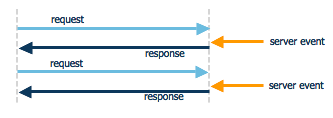
\includegraphics[height=0.15\textheight]{assets/images/theoretical2/http_schema.png}
  \caption{Упрощённая схема клиент-серверного взаимодействия при использовании протокола HTTP}
  \label{img:http__schema}
\end{figure}

Одним из основных архитектурных стилей взаимодействия распределённых приложений в сети является REST (REpresentational State Transfer, передача состояния представления). Программные интерфейсы приложения (API), придерживающиеся принципов REST называются RESTful API. REST API используют модель запрос/ответ, при которой каждое сообщение от сервера является ответом на сообщение от клиента~\cite{http_websockets}. В основном, RESTful API используют протокол HTTP в качестве транспортного. В зависимости от цели, запросы в REST делятся на GET, PUT, POST и DELETE, которые используются для получения, изменения, создания и удаления данных соответственно.

Протокол WebSocket предоставляет возможность как клиенту, так и серверу отправлять сообщения, не основываясь на истории предыдущих запросов. В настоящее время практически все браузеры поддерживают WebSocket.

WebSocket позволяет решить несколько проблем, возникающих при использовании протокола HTTP~\cite{http_websockets}:

\begin{enumerate}
  \item Двунаправленность протокола --- и клиент, и сервер имеют возможность отправлять сообщения друг другу. Используя HTTP, запрос всегда инициируется клиентом, а ответ всегда производится сервером, что делает HTTP однонаправленным протоколом;
  \item Полнодуплексная коммуникация --- обмен сообщениями между клиентом и сервером происходят независимо и одновременно;
  \item Одно TCP соединение --- после установления HTTP соединения в начале, клиент и сервер обмениваются сообщениями по одному TCP соединению в течение всего времени существования WebSocket соединения. 
\end{enumerate}

На рисунке~\ref{img:webSocket__schema} представлена упрощённая схема WebSocket соединения.

\begin{figure}[H]
  \centering
  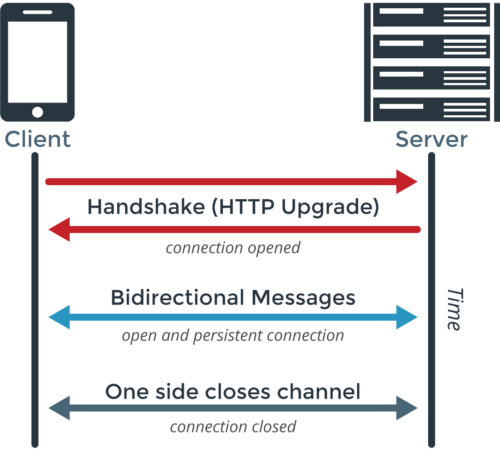
\includegraphics[height=0.2\textheight]{assets/images/theoretical2/webSocket_schema.png}
  \caption{Упрощённая схема WebSocket соединения}
  \label{img:webSocket__schema}
\end{figure}

Было произведены тесты, сравнивающие производительность REST и WebSocket соединений~\cite{http_websockets}. Тесты производились для как для различного количества запросов к серверу, так и для различной нагрузки. В таблице~\ref{tab:constant_payload} представлены результаты тестов REST и WebSocket соединений при одинаковой нагрузке запросов, в таблице~\ref{tab:increasing_payload} результаты тестов REST и WebSocket соединений при одинаковом количестве запросов, но различной нагрузке сообщений.

\begin{table}[H]
  \caption{Результаты тестов REST и WebSocket соединений при одинаковой нагрузке запросов}
  \label{tab:constant_payload}
  \begin{tabular}{|c|r|r|r|}
  \hline
  \textbf{Запросов} & \textbf{REST, мс} & \textbf{WebSocket, мс} & \textbf{Разница, раз} \\ \hline
  10    & 17    & 13   & 1,31  \\ \hline
  100   & 112   & 20   & 5,60  \\ \hline
  500   & 529   & 68   & 7,78  \\ \hline
  1000  & 1050  & 115  & 9,13  \\ \hline
  5000  & 5183  & 522  & 9,93  \\ \hline
  10000 & 10547 & 1019 & 10,35 \\ \hline
  \end{tabular}
\end{table}

\begin{table}[H]
  \caption{Результаты тестов REST и WebSocket соединений при одинаковом количестве запросов, но различной нагрузке сообщений}
  \label{tab:increasing_payload}
  \begin{tabular}{|c|r|r|r|}
  \hline
  \textbf{Нагрузка} & \textbf{REST, мс} & \textbf{WebSocket, мс} & \textbf{Разница, раз} \\ \hline
  10    & 1003 & 81  & 12,38 \\ \hline
  100   & 1013 & 87  & 11,64 \\ \hline
  500   & 1032 & 113 & 9,13  \\ \hline
  1000  & 1044 & 119 & 8,77  \\ \hline
  5000  & 1173 & 243 & 4,83  \\ \hline
  10000 & 1289 & 394 & 3,27  \\ \hline
  \end{tabular}
\end{table}

Исходя из данных, полученных в результате тестов, можно сделать вывод, что WebSocket предпочтителен в случае использования приложений, где важна скорость получения новых данных клиентом и использование наименьшего количества ресурсов сервера для обработки запроса. Преимущество WebSocket над REST объяснимо тем, что при каждом REST запросе создаётся новое TCP соединение, удовлетворяющее семантике HTTP~\cite{http_websockets}.
